% this file is called up by thesis.tex
% content in this file will be fed into the main document

%: ----------------------- name of chapter  -------------------------

\chapter{Literature Survey} % top level followed by section, subsection

%: ----------------------- paths to graphics ------------------------

% change according to folder and file names
\ifpdf
    \graphicspath{{2_LiteratureSurvey/figures/PNG/}{2_LiteratureSurvey/figures/PDF/}{2_LiteratureSurvey/figures/}}
\else
    \graphicspath{{2_LiteratureSurvey/figures/EPS/}{2_LiteratureSurvey/figures/}}
\fi

%: ----------------------- contents from here ------------------------

This chapter will provide the background that will help to put the research conducted in this thesis into context. The four broad areas of study will be regarding the HER2 biomarker and its scoring criteria, previous attempts at generating HER2 IHC stain images followed by an introductory study of Stable Diffusion and ControlNet which will be the main focus in Chapter 3 i.e., the methodology and implementation for this research.

\section{HER2 in Breast Cancer}

As briefly mentioned in the introduction section, the Human Epidermal Growth Factor Receptor 2 (HER2) influences both tumor aggressiveness and treatment outcomes making this a critical factor in the pathology of breast cancer \parencite{Moasser2007ThePathogenesis.}. The HER2 receptor gene promotes cell proliferation and survival. Intuitively, when this is over-expressed, it has the same effect on tumor cells leading to its aggressive spread. Amplification or over-expression of the HER2 gene occurs in approximately 15-20\% of breast cancers  \parencite{Slamon1987HumanOncogene.}  and is associated with poor prognosis and increased risk of recurrence. However, HER2 also represents a potent target for targeted therapies such as trastuzumab  \parencite{Slamon2001UseHER2}  that have significantly improved survival outcomes in HER2-positive breast cancer patients \parencite{Perez2014TrastuzumabN9831}.

\subsection{HER2 Testing and IHC Scoring}

The most common method for assessing the HER2 amplification status is immunohistochemistry (IHC) which detects the HER2 gene overexpression in tissue samples by method of staining. The IHC scoring system grades staining intensity in tumor cells ranging from 0 (negative) to 3+ (positive). The two scores in between i.e., 1+ and 2+ indicate low expression and equivocal expression respectively with the latter typically requiring confirmation through another test called in situ hybridization (ISH) \parencite{Ivanova2024StandardizedCancer.}. This is further corroborated by  \textcite{Wolff2018HumanUpdate}, who assert that this scoring system is central in the clinical guidelines by the American Society of Clinical Oncology (ASCO) and College of American Pathologists (CAP) to standardize diagnostic procedures in different laboratories. The guidelines specify the criteria for each IHC score, providing a framework for determining the HER2 IHC  score and recommending ISH as a follow-up test for borderline cases. The test scores and corresponding criteria for the scoring are detailed in Table \ref{tab:HER2 IHC Scoring Guidelines}. 

\begin{table}[H]
\begin{center}
\begin{tabular}{|p{0.07\linewidth}|>{\raggedright\arraybackslash}p{0.7\linewidth}|>{\raggedright\arraybackslash}p{0.23\linewidth}|}
\hline 
\textbf{IHC Score}& \textbf{Staining Pattern/Scoring Criteria}& \textbf{HER2 Expression}\\ \hline 
0& No staining or incomplete and faint/barely perceptible membrane staining in $\leq 10 \% $ of tumor cells.& Negative\\ \hline
1+& Incomplete and faint/barely perceptible membrane staining in $> 10\%$ tumor cells.&  Low expression\\ \hline
2+& Weak to moderate complete membrane staining in $>10\%$ of tumor cells OR intense membrane staining in $\leq 10\%$ of tumor cells.& Equivocal (low expression if slide is ISH-negative, positive if ISH-positive.)\\ \hline
 3+& Complete and intense membrane staining in $> 10\%$ of tumor cells.&Positive\\\hline
\end{tabular}
\caption[HER2 Scoring Guidelines]{HER2 Scoring Guidelines according to ASCO/CAP guidelines \parencite{Ivanova2024StandardizedCancer.}}\label{tab:HER2 IHC Scoring Guidelines}
\end{center}
\end{table}
\vspace{5mm}

\subsection{{Problems with Manual IHC Scoring}}

Despite the consistent framework that is in place for HER2 scoring, the evaluation of cases comes down to the judgement of human pathologists which leads to manual scoring being subjective on account of inter-observer variability and diagnostic discrepancies. This variability has direct implications for treatment decisions. Inaccurate classification of HER2 status can lead to sub-optimal therapeutic choices, such as the exclusion of eligible patients from receiving trastuzumab or the unnecessary administration of HER2-targeted therapies to those unlikely to benefit.

As a consequence of the known subjectivity, this also puts pressure on the pathologists to get it right given the potential ramifications which inadvertently makes the already labour intensive manual scoring process more time-consuming as pathologists ensure the process is given the careful attention that is required. A tool that could provide instant IHC scores from the more easily and cheaply producible H\&E stain while also providing a digitally stained IHC image with high accuracy for pathologists to review would make the lives of pathologists a lot more easier giving them a reference point to know what to expect. This is precisely the aim for this thesis and other previous research on this subject.

\section{State-of-the-Art in IHC Stain Generation}

Recent work and application of deep neural networks to the field of histopathological analysis has opened new avenues for improving efficiency and accuracy. The idea of generating IHC stains from the traditional H\&E stained slide images is not new. Generative adversarial networks (GANs) have proven to be a popular choice of network architecture for stain transfer and has yielded promising results as surveyed by \textcite{Srinidhi2021DeepSurvey} where they show seven out of eight research studies using GANNs or a variation of them for this task.

\subsection{Application of GANs}

The landmark work of  \textcite{Goodfellow2014GenerativeNetworks}  introduced Generative Adversarial Networks that has been instrumental in the generative AI space. A GAN architecture has two neural networks, a generator and a discriminator,. They compete in a zero-sum game where the generator creates synthetic data that tries to imitate real data while the discriminator attempts to identify the real and generated synthetic data. This competition between the networks leads to the production of highly realistic generated data that have seen its use in image generation, data augmentation and even video generation tasks. 

\subsubsection{CycleGAN}

There have been many variations and alternative architectures of the original GAN architecture that have significantly advanced the generative AI field \parencite{Goodfellow2020GenerativeNetworks}. For the task of stain transfer in particular, \textbf{CycleGANs} have been a popular architecture of choice because it allows for unpaired image-to-image translation. In other words, CycleGAN provides the ability to learn mappings from one domain to another domain such as from H\&E stained slides to IHC stained slides without the need for paired data \parencite{Zhu2017UnpairedNetworks}. It can do this because it has two generator-discriminator pairs which uses the "cycle consistency" rule which forces the model to be able to transform an image to another domain or style and back again, ensuring the transformation makes sense both ways. This is illustrated in Figure \ref{fig:CycleGAN} . This makes it a good fit for areas like histopathology stain transfer research where obtaining directly paired images is difficult. That being said, when paired labelled data is available, that would inherently be more advantageous for a model to learn from because it has obvious direct targets to learn to mimic.

\begin{figure}[h]
    \centering
    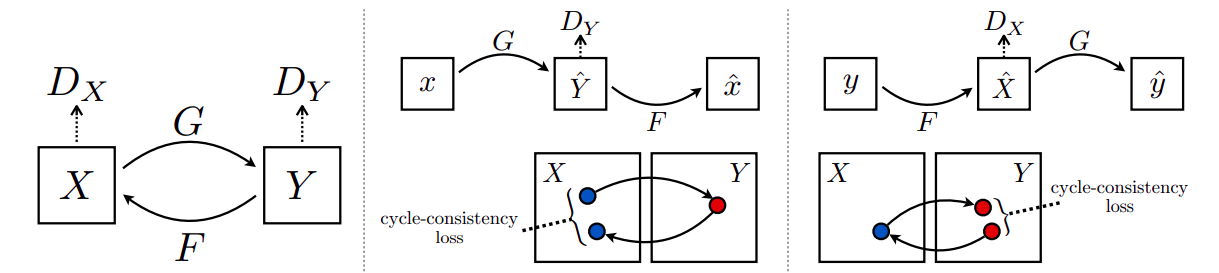
\includegraphics[width=1.0\linewidth]{2_LiteratureSurvey/figures/CycleGAN.png}
    \caption[CycleGAN workflow]{Illustration of CycleGAN's working where $G \& F$ are generators, $D_{X} \& D_{Y}$ are discriminators and $X \& Y$ represent the domains between whom mapping is to be learnt \parencite[Figure 3, p. 2244]{Zhu2017UnpairedNetworks}.}
    \label{fig:CycleGAN}
\end{figure}

\subsubsection{pix2pix}

With paired datasets in mind the \textbf{pix2pix} model has seen some extensive use in stain transfer research. It was first introduced by  \textcite{Isola2016Image-to-ImageNetworks} as a type of \textit{conditional} GAN (cGAN) which by nature means it is used for paired image-to-image translation tasks like converting edge maps into photo-realistic renders. This model also has the generator and discriminator setup but rather than being traditional networks, the generator is a \textbf{U-Net} style architecture which is also employed in Stable Diffusion models with encoding and decoding layers. It also allows \textit{skip-connections} between these layers which enables the model to retain low-level details from the input image while generating the output. The discriminator is a \textit{PatchGAN} which classifies patches of the image as either real or fake instead of the entire image. This allows for higher focus on the local details in image such as texture, structural patterns and so on. Also, unlike in CycleGANs, the input signal is used by both the generator and discriminator due to the paired nature of data used (Figure \ref{fig:pix2pix}). Thus the discriminator is more adept at challenging the generator ultimately resulting in much higher quality outputs.

\begin{figure}[h]
    \centering
    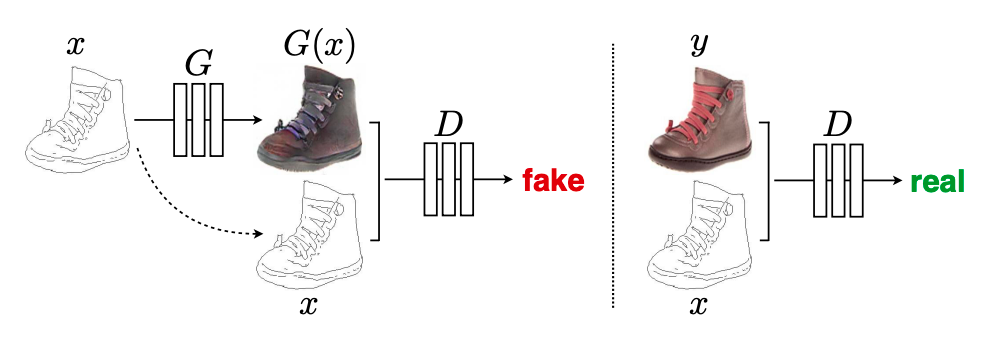
\includegraphics[width=1\linewidth]{2_LiteratureSurvey/figures/pix2pix.png}
    \caption[pix2pix workflow]{The pix2pix training workflow as illustrated in \parencite[Figure 2, p. 2]{Isola2016Image-to-ImageNetworks}}
    \label{fig:pix2pix}
\end{figure}
In terms of performance in H\&E stain to HER2 IHC stain transfer, pix2pix models show better results than CycleGAN when comparing objective evaluation metrics such as the Peak Signal to Noise Ratio (PSNR) and Structural Similarity (SSIM) for assessing the quality of the image \parencite[Table 1, p. 7]{Liu2022BCI:Pix2pix}.

\subsubsection{Pyramid pix2pix}

This refinement on the pix2pix approach proposed by  \textcite{Liu2022BCI:Pix2pix}  is some of the latest research in this niche but fast emerging field of stain transfer. It also makes the Breast Cancer Immunohistochemical (BCI) dataset available that is used train our models on. This dataset is not only a paired H\&E-IHC dataset but is also processed such that the image patches are registered and aligned at a structural level. However, because the stains are of different domains a lot of positions cannot achieve pixel-level alignment. For example, in Figure \ref{fig:he-ihc-alignment-issue-example} we can see that there is clear presence of fat tissue towards the centre-right of the IHC image patch where there are white globule like structures but it is not significantly present in the H\&E image patch.

\begin{figure}[h]
    \centering
    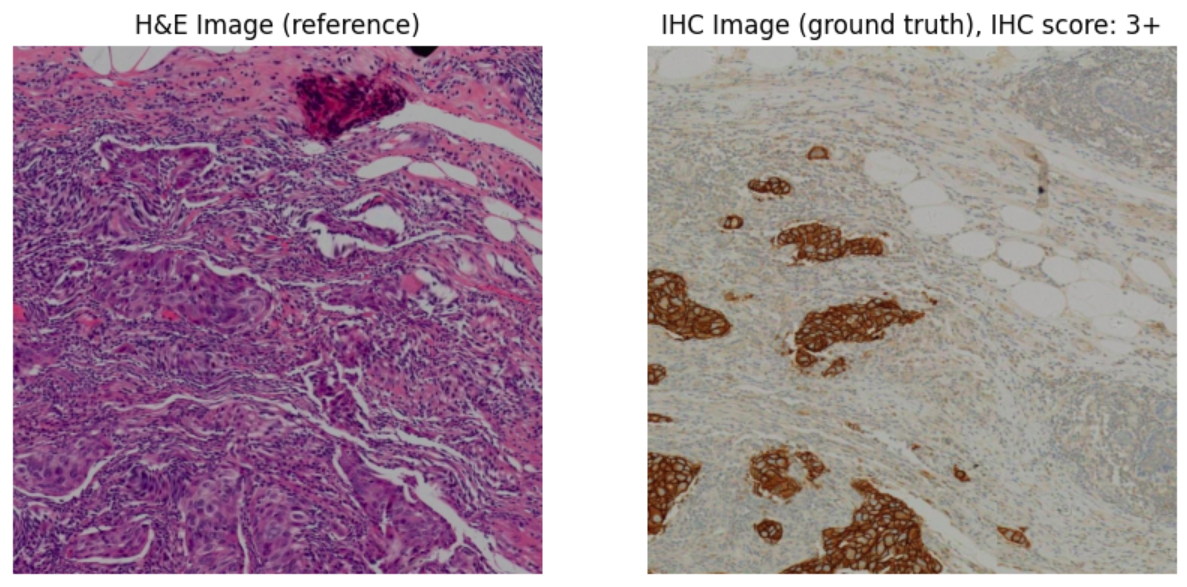
\includegraphics[width=1\linewidth]{2_LiteratureSurvey/figures/he-ihc-alignmentIssue.png}
    \caption{H\&E-IHC discrepancy in structural alignment}
    \label{fig:he-ihc-alignment-issue-example}
\end{figure}
Given that traditional pix2pix models work best with image-pairs that have good pixel-level alignment (which is why often the inputs are image maps like edges), the Pyramid pix2pix approach modifies the loss function by performing scale transformation on the ground truth images and the corresponding image that is generated by the generator network. The performed transformation smooths and down-samples the image making it blurred and of lower resolution. The transformation is done over multiple steps and the loss at each step is calculated. The higher the dimension, the closer to the ground truth the generated image can get due to increasing blur and down-sampling. The sum of the products of  loss at each scale, $S_{i}$ and the weight of the scale, $\lambda_{i}$ makes up the multi-scale loss which is then added to the overall loss function where $i$ is the scale  \parencite[Equation 2, p. 6]{Liu2022BCI:Pix2pix}. 
\begin{equation}\label{eq:multi-scale-loss}
L_{multi−scale} = \sum_{i}^{} \lambda_{i}S_{i}
\end{equation}
This strategy proves to have worked in their own benchmarks where the Pyramid pix2pix model show the best results when compared against traditional variations of pix2pix and also CycleGAN \parencite[Table 1, p. 7]{Liu2022BCI:Pix2pix}.  

\section{Stable Diffusion}



\section{ControlNet}

Lorem ipsum dolorem


% ---------------------------------------------------------------------------
%: ----------------------- end of Literature Review chapter ------------------------
% ---------------------------------------------------------------------------

